\documentclass{article}


\usepackage{arxiv}

\usepackage[utf8]{inputenc} % allow utf-8 input
\usepackage[T1]{fontenc}    % use 8-bit T1 fonts
\usepackage{hyperref}       % hyperlinks
\usepackage{url}            % simple URL typesetting
\usepackage{booktabs}       % professional-quality tables
\usepackage{amsfonts}       % blackboard math symbols
\usepackage{nicefrac}       % compact symbols for 1/2, etc.
\usepackage{microtype}      % microtypography
\usepackage{lipsum}
\usepackage[polish]{babel} % English language hyphenation
\usepackage{float} % for H in \begin{figure}[H]. Force including file in place.

\usepackage{graphicx}
\graphicspath{ {./images/} }


% kolory odnośników
\usepackage[dvipsnames]{xcolor}
\hypersetup{
    colorlinks=true,
    linkcolor=black,
    filecolor=black,
    citecolor=black,
    urlcolor=cyan,
    pdftitle={Sharelatex Example},
    pdfpagemode=FullScreen,
}
\urlstyle{same}


\title{Kwantyzacja wektorowa}

\author{
  Karol Działowski \\
  \textbf{Wojciech Olejnik} \\
  \textbf{Paweł Kalicki} \\
  Zachodniopomorski Uniwersytet Technologiczny
}

\begin{document}
\maketitle
\begin{abstract}
Automaty komórkowe są powszechnie używanym narzędziem wykorzystywanym do budowania modeli, ze względu na ich prostotę, oraz łatwość przeprowadzania na nich badań. W poniższej pracy wykorzystano teorię automatów komórkowych do zaprojektowania i implementacji niezbędnych modeli dróg, które następnie wykorzystano do modelowania układu ruchu drogowego w celu zbadania czynników wpływających na powstawanie zatorów drogowych. Badaniom poddano układy komunikacyjne o różnych wielkościach, wykorzystujące różne modele dróg. Do implementacji aplikacji wykorzystano język programowania Python.
\end{abstract}


% keywords can be removed
%\keywords{First keyword \and Second keyword \and More}


\section{Wstęp}
W ostatnich latach symulacje ruchu drogowego zyskały na znaczeniu ze względu na możliwości badań systemów komunikacyjnych. Takie modele najczęściej implementowane są przy użyciu automatów komórkowych. Automaty komórkowe (\emph{ang. cellular automata}) zostały pierwszy raz użyte przez Johanna Louisa von Neumanna w badaniach nad żywymi biologicznymi systemami, co zostało udokumentowane w jego pracy z 1948 roku. \cite{von1948} Najpopularniejszym przykładem użycia automatów komórkowych jest ,,Game of Life'' Johna Conwaya. \cite{games1970fantastic}

Automaty komórkowe są systemami, które składają się z siatki komórek przyjmujących jeden z ustalonych stanów. Zachowania każdego elementu są zależne od stanu sąsiadujących komórek. W trakcie symulacji wszystkie komórki aktualizują swój stan w pojedynczym kroku. Służą do modelowania układów dynamicznych, które umożliwiają badanie wpływu różnych czynników na badany model. W tym przypadku automat komórkowy zostanie wykorzystany do modelowania ruchu drogowego.

Do modelowania ruchu drogowego wykorzystywane są modele stochastyczne. Podstawowy model zaproponowany w 1992 roku przez Nagela i Schreckenberga pozwala na odtworzenie tworzenia się spontanicznych zatorów drogowych na jednokierunkowej drodze. \cite{nagel1992cellular} Model ten, nazywany STCA (\emph{ang. stochastic traffic cellular automaton}) jednoznacznie określa zasadę losowości, gdzie z danym prawdopodobieństwem zmieniana jest prędkość pojazdu, co symuluje pewne sytuacje na drodze czy zachowania kierowców.

Modele pojedynczych pasów nie są zdolne do symulowania realistycznego ruchu drogowego z prostego powodu. Wprowadzając auta o różnych charakterystykach (różnych prędkościach) w symulacji występuje zjawisko zbieżności do prędkości auta najwolniejszego. Wykorzystanie modelu dwupasmowego wyeliminowało ten problem. Dzięki dwóm równoległym pasom i dodatkowym zasadom możliwe jest wyprzedzanie aut wolniejszych. \cite{rickert1996two}

wcześniej przytoczone modele dobrze nadają się do modelowania i badania ruchu na autostradach. W celu symulacji skomplikowanych systemów należy wprowadzić nowe modele. Systemy skrzyżowań powszechnie występują w systemach ruchu miejskiego. Odgrywają ważną rolę w sterowaniu całego systemu ruchu drogowego. \cite{wu2005study}

Modele skrzyżowań możemy podzielić ze względu na kształt skrzyżowań (skrzyżowania typu T oraz skrzyżowania typu X) oraz ze względu na sygnalizację na skrzyżowaniach (brak sygnalizacji z określonymi drogami z pierwszeństwem i podporządkowanymi oraz skrzyżowania z sygnalizacją świetlną).

Większość skrzyżowań bez sygnalizacji świetlnej w systemach ruchu drogowego jest typu T. \cite{wu2005study} Skrzyżowanie to składa się z połączenia dwóch dróg, gdzie jedna jest podporządkowana i kończy się skrętem a druga jest uprzywilejowana. Liczne prace określają takie modele, gdzie wprowadzane są dodatkowe reguły zmiany kierunku ruchu i rozstrzygania konfliktów.  \cite{wu2005study, li2009cellular}

Podobne modele opisują skrzyżowania typu X. Takie skrzyżowanie składa się z dwóch prostopadłych,przecinających się prostych odcinków. W modelach uwzględniono różne podejścia i schematy skrzyżowań. Są to skrzyżowania tylko o skrętach w prawo (bezkolizyjne), czy skrzyżowania tylko z jednym skrętem w lewo, lub pełne skrzyżowania. \cite{marzoug2014cellular}

Ronda są popularnym rozwiązaniem redukcji zatorów drogowych dlatego powinny zostać odpowiednio zaprojektowane podczas modelowania ruchu drogowego. \cite{marzoug2014cellular} Podstawowym problemem w modelowaniu skrzyżowań o ruchu okrężnym jest określenie jaki warunek musi być spełniony, aby model auta mógł wjechać na rondo. \cite{campari2004cellular} Przykładowym warunkiem jest sprawdzenie czy przestrzeń między wjazdem na rondo, a poprzednim wjazdem jest pusta. \cite{campari2004cellular, wang2005realistic}

Celem projektu była budowa aplikacji umożliwiającej budowanie dowolnego układu komunikacyjnego z przetestowaniem efektywności różnych konfiguracji sterowania ruchem drogowym. Poszczególne elementy zrealizowano w postaci obiektowej umożliwiając składanie ich i budowanie większych obiektów. Zaimplementowano wyżej wymienione schematy połączeń, to znaczy odcinek prosty jedno i wielopasmowy, skrzyżowania typu T, X bez sygnalizacji oraz z sygnalizacją oraz ronda.

\section{Opis projektu}

Celem projektu było stworzenie aplikacji umożliwiającej budowanie dowolnego układu komunikacyjnego za pomocą prostych obiektów dróg. Podstawowe modele dróg zaimplementowane w aplikacji:
\begin{itemize}
    \item Odcinek prosty jednopasmowy.
    \item Skrzyżowanie typu T.
    \item Skrzyżowanie typu X.
    \item Skrzyżowania typu T oraz X ze światłami.
    \item Rondo.
\end{itemize}
\subsection{Modele dróg}
Wszystkie podstawowe modele dróg zaimplementowane w aplikacji posiadają własną siatkę komórek, z których następnie określane są komórki należące do drogi. Każda z komórek będąca fragmentem drogi ma zapisany kierunek z jakim będą poruszać się auta znajdujące się na niej. W przypadku gdy dwie lub więcej dróg łączą się ze sobą tworzona jest lista kierunków, z których następnie auto wybiera z określonym prawdopodobieństwem, w którą stronę będzie jechać.
\begin{figure}[h]
    \centering
    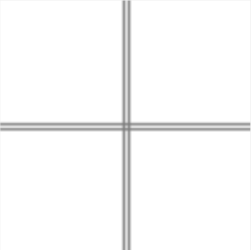
\includegraphics[width=0.3\textwidth]{images/skrzyzowanie.png}
    \caption{Przykładowy model drogi. Skrzyżowanie typu X.}
    \label{fig:crossing}
\end{figure}
\subsection{Model auta}
Obiekt auta zaimplementowany w projekcie posiada następujące właściwości:
\begin{itemize}
    \item Pozycja zapisana jako wektor 2D - Przechowuje aktualne współrzędne auta na mapie.
    \item Prędkość w skali od 0 do 4 - Określa o ile komórek dane auto może się poruszyć w trakcie jednej iteracji symulacji.
    \item Kierunek jazdy zapisany jako wektor 2D - Przechowuje informacje o aktualnym kierunku jazdy.
\end{itemize}
W trakcie trwania symulacji każde auto aktualizuje swoją pozycję przesuwając się o ilość komórek określoną prędkością wzdłuż obranego kierunku jazdy. Jeżeli przeskok o daną ilość komórek jest niemożliwy ze względu na auto znajdujące się na drodze, które porusza się wolniej, prędkość jest redukowana.
\subsection{Interfejs graficzny}
Na potrzeby aplikacji stworzono interfejs umożliwiający umieszczanie poszczególnych modeli na mapie oraz łączenie ich w jeden układ co umożliwiło przemieszczanie się aut płynnie z jednej drogi na drugą. 
\begin{figure}[h]
    \centering
    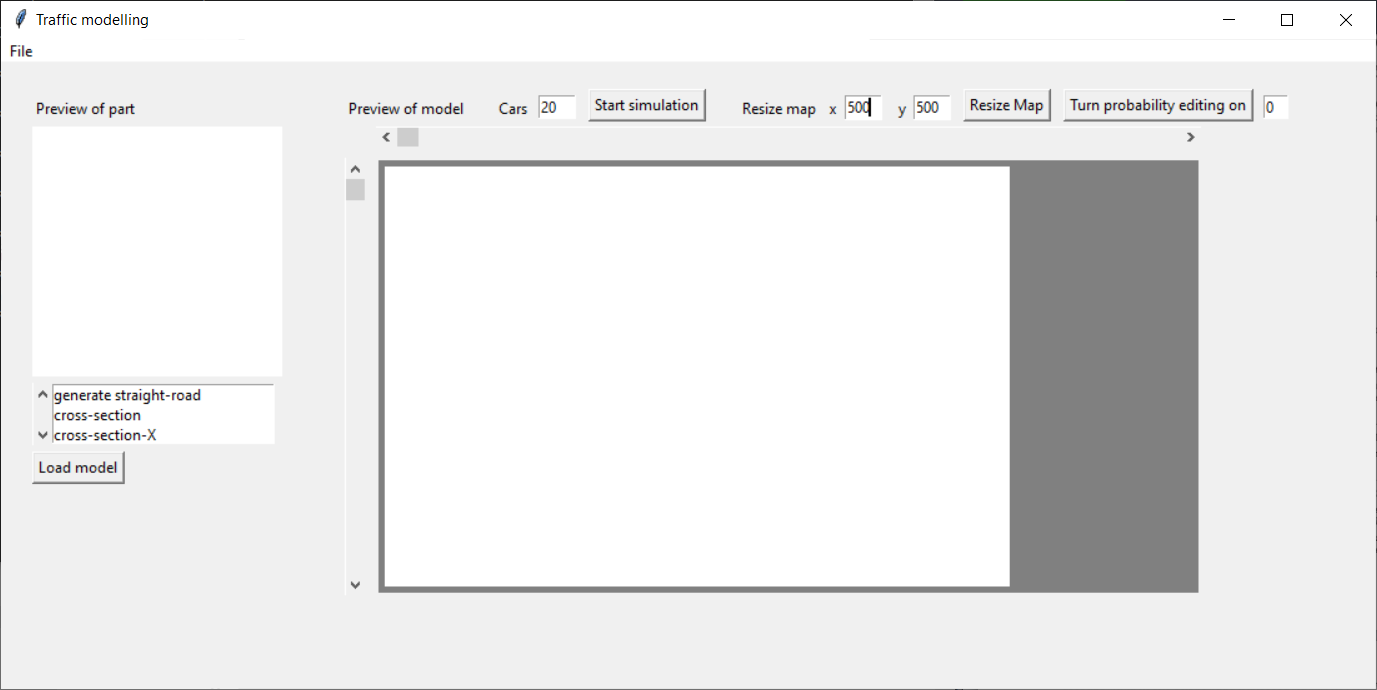
\includegraphics[width=0.8\textwidth]{images/gui.PNG}
    \caption{Interfejs graficzny aplikacji.}
    \label{fig:gui}
\end{figure} \\
Zaimplementowany interfejs graficzny pokazany na rysunku \ref{fig:gui} pozwala zmieniać liczbę samochodów na mapie, które są generowane w trakcie trwania symulacji. Mapa jest elementem, którego wielkość można dostosowywać do potrzeb symulacji w trakcie budowania modelu. Dodatkowo istnieje możliwość edycji prawdopodobieństwa skrętu na danej drodzy z poziomu aplikacji co pozwala na modelowanie zatłoczonych ulic i symulowanie korków ulicznych.

\section{Przeprowadzone badania}

Zaimplementowana aplikacja pozwala na przeprowadzenie kilku rodzaju badań. Zbierane są dane o prędkościach każdego z samochodów i zapisywane w postaci plików \emph{csv}. Oprócz tego generowane są mapy cieplne badanych układów. 

Jedna mapa ciepła pokazuje ogólny rozkład ruchu w systemie a druga mapa ciepła przedstawia rozkład miejsc w których występowały zatory. Wizualizacje te pozwalają na łatwą identyfikację wąskich gardeł (\emph{ang. bottleneck}) w badanych systemach.

\subsection{Mały układ}

Pierwszy badany układ (rysunek \ref{fig:model_maly}) zbudowany został zbudowany z prostych odcinków dwukierunkowych i skrzyżowań. W centrum modelu znajduje się skrzyżowanie typu T bez sygnalizacji świetlnej, które jest połączone z dwoma skrzyżowaniami typu T z światłami oraz jednym skrzyżowaniem typu X. 

\begin{figure}[H]
    \centering
    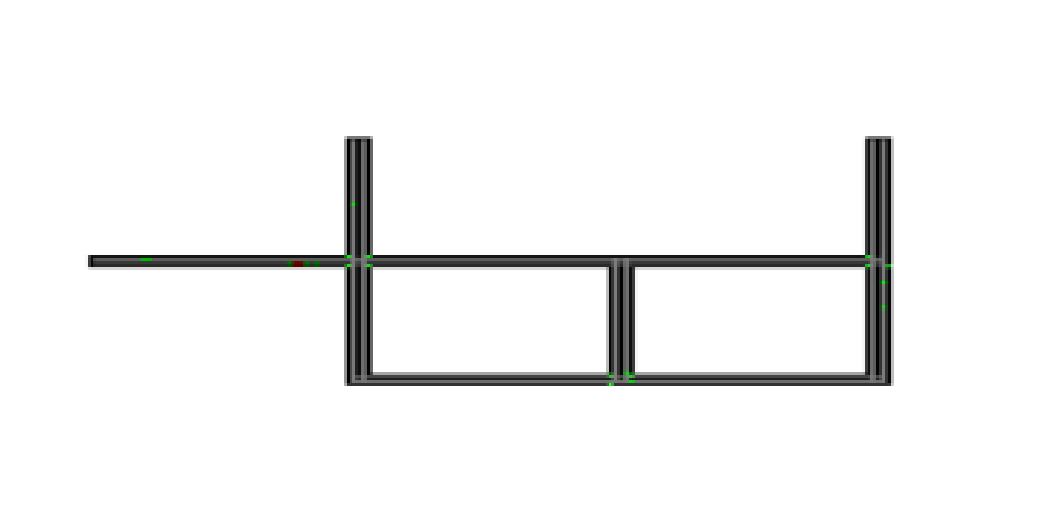
\includegraphics[width=0.5\textwidth]{images/modele/small.png}
    \caption{Model 1}
    \label{fig:model_maly}
\end{figure}

Badanie trwało 2000 iteracji i w symulacji brało udział 50 aut. Dla każdego auta zebrano dane o jego prędkości w czasie. Wykonano również wykres czasowo przestrzenny i mapy cieplne. 

Dane w postaci wizualizacji przedstawiono na wykresie (\ref{fig:dane_maly}). Większość ruchu przeprowadzana była dolnym odcinkiem, czyli z pominięciem skrzyżowania T bez sygnalizacji. Największe korki pojawiały się w prawej części modelu, na odcinku ze skrzyżowaniem T z sygnalizacją.

\begin{figure}[H]
    \centering
    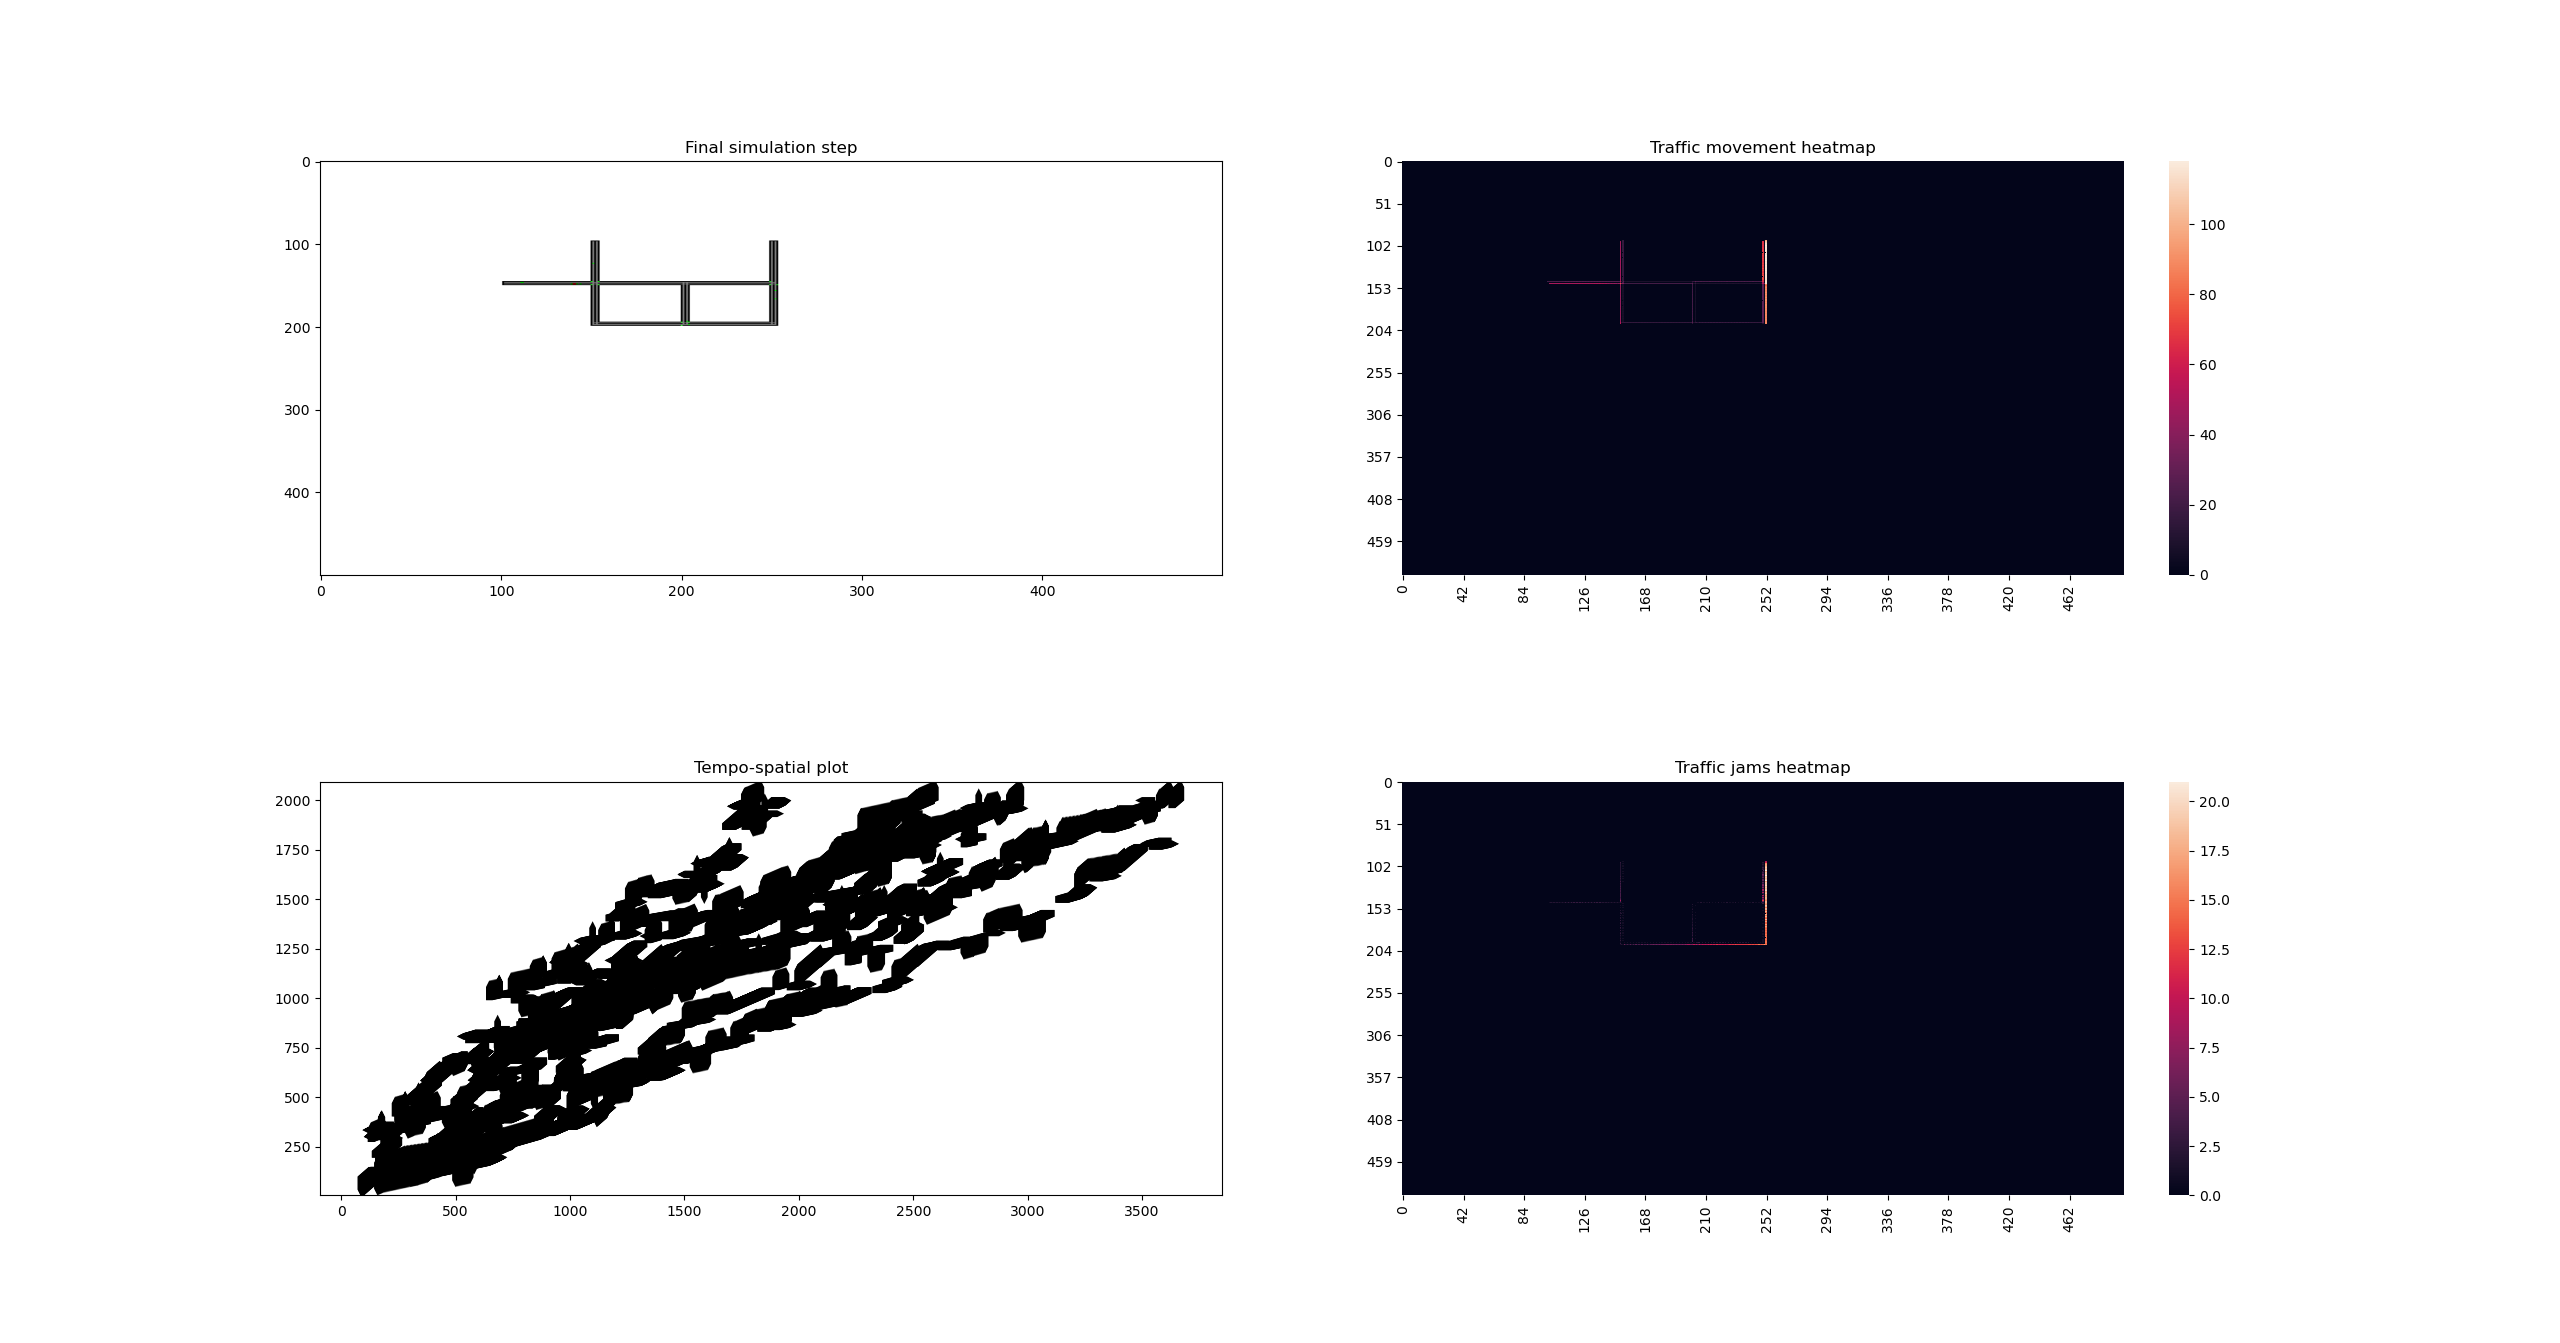
\includegraphics[width=0.8\textwidth]{images/Figure_1.png}
    \caption{Zebrane dane dla modelu 1}
    \label{fig:dane_maly}
\end{figure}


\subsection{Średni układ}

Drugi badany układ (rysunek \ref{fig:model_sredni}) zbudowany został z większej ilości skrzyżowań, przypominający układ ulic Nowego Jorku. Układ składa się z trzech głównych dróg ustawionych pionowo, które są połączone drogami poprzecznymi. W układzie na skrzyżowaniach typu X zewnętrznych dróg głównych wykorzystano sygnalizację świetlną.

\begin{figure}[H]
    \centering
    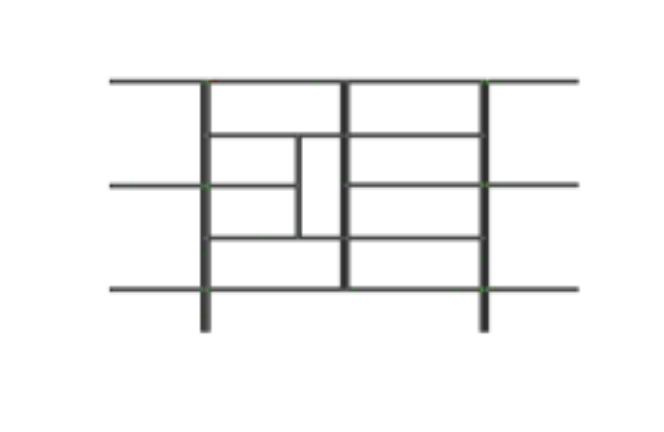
\includegraphics[width=0.5\textwidth]{images/modele/medium.png}
    \caption{Model 2}
    \label{fig:model_sredni}
\end{figure}

 Badanie przeprowadzono na 2000 iteracjach i zebrano dane o prędkości dla 50 aut. W tym przypadku nie wykonano wykresu czasowo przestrzennego ze względu na długość obliczeń. 
 
 Zebrane dane przedstawiono na wykresie (\ref{fig:dane_sredni}). Na podstawie mapy cieplnej możemy dowiedzieć się o rozkładzie ruchu na badanym systemie. Najczęściej uczęszczana była droga pozioma znajdująca się na górze symulacji, która łączyła wszystkie trzy drogi główne. Środkowa droga główna była mało uczęszczana przez samochody. Taka sytuacja powstała w wyniku odpowiedniego doboru prawdopodobieństw wyboru dróg przez samochody. 
 
Mapa zatorów w badanym systemie jest analogiczna do mapy zagęszczenia ruchu. Korki występują tam gdzie było największe natężenie samochodów, czyli w górnym poziomym odcinku łączącym drogi główne.
 
 \begin{figure}[H]
    \centering
    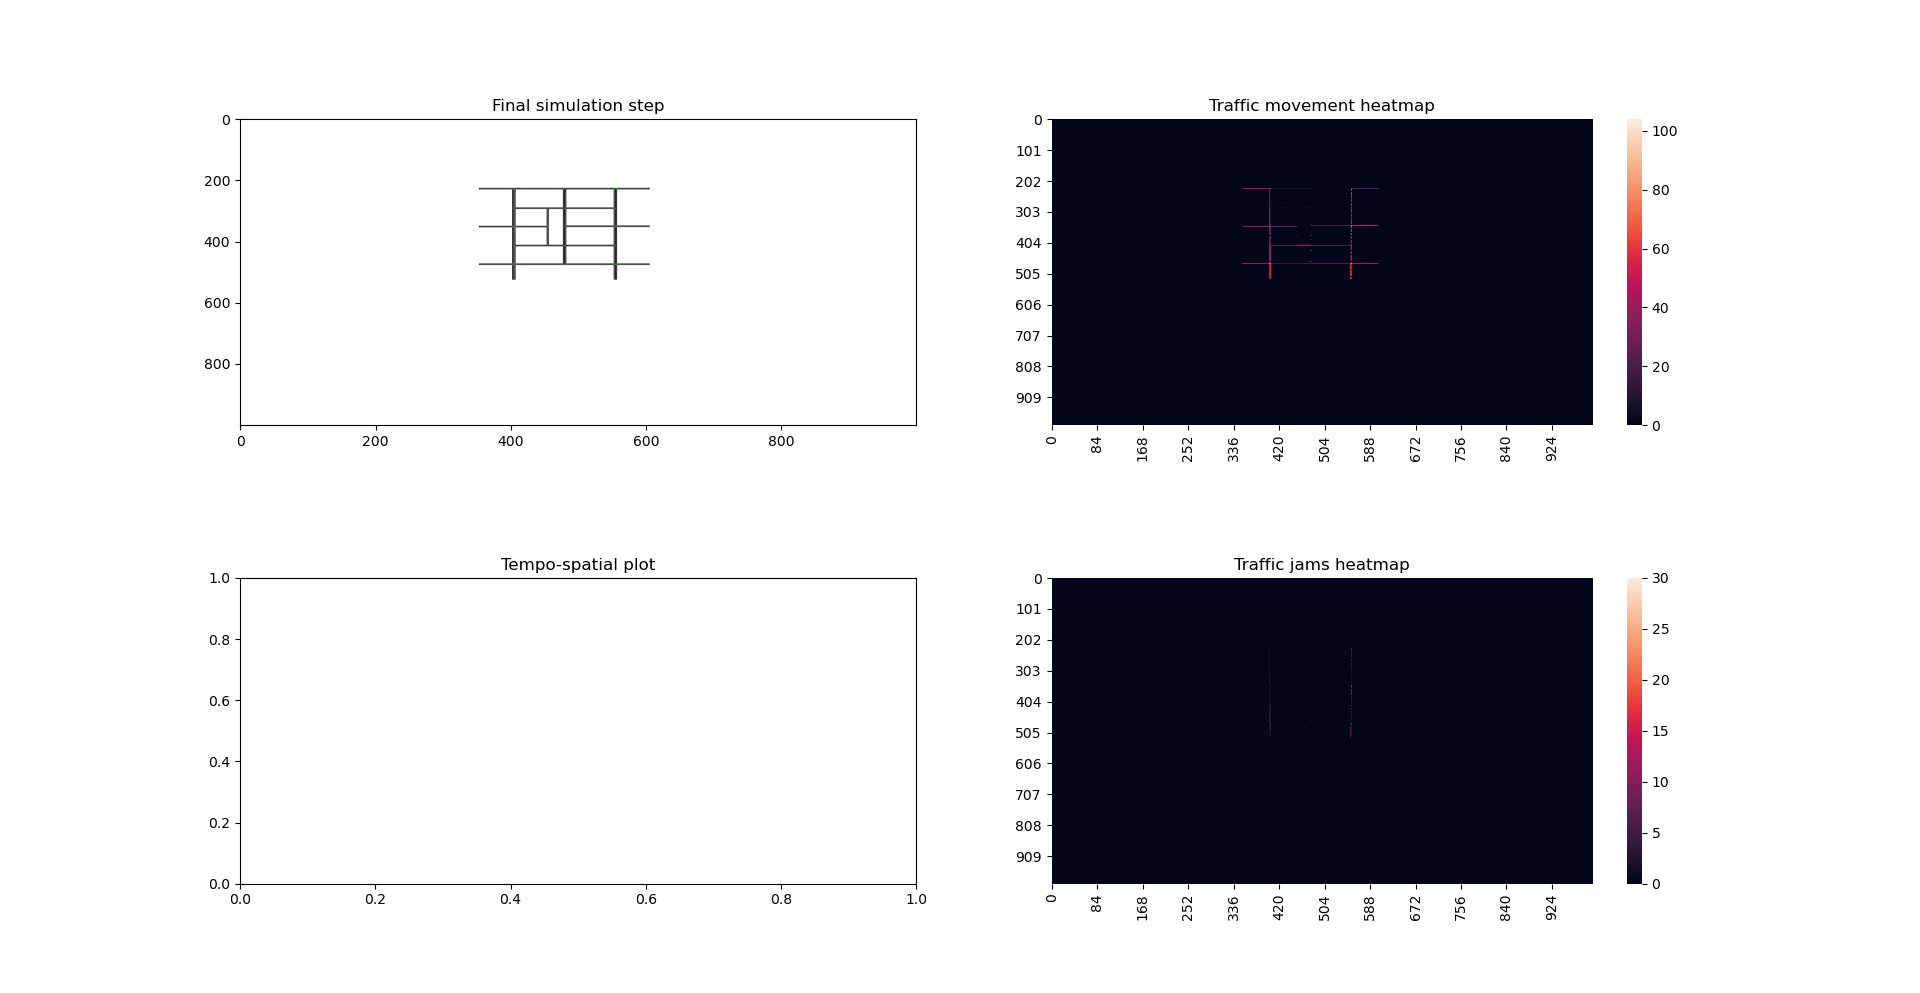
\includegraphics[width=1\textwidth]{images/medium_model.png}
    \caption{Zebrane dane dla modelu 2}
    \label{fig:dane_sredni}
\end{figure}

\subsection{Duży układ}

Ostatni badany układ (rysunek \ref{fig:model_duzy}) jest najbardziej kompleksowym z badanych układów. Jego składowymi są drogi poprzeczne, skrzyżowania tupu T z sygnalizacją i bez sygnalizacji oraz ronda. 

\begin{figure}[H]
    \centering
    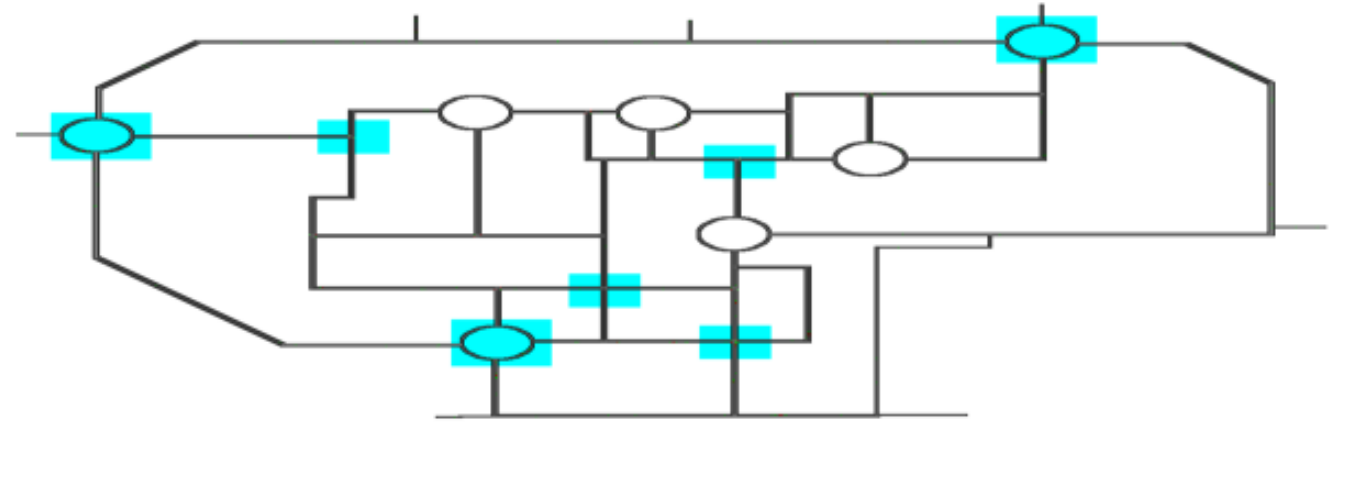
\includegraphics[width=0.6\textwidth]{images/modele/large.png}
    \caption{Model 3}
    \label{fig:model_duzy}
\end{figure}

Badanie przeprowadzono dla 2000 iteracji. Zebrano informacje o prędkościach aut i zapisano je do plików \emph{csv}. Wizualizacje zebranych danych przedstawiono na wykresie (\ref{fig:dane_duzy}). Z mapy cieplnej można wywnioskować rozłożenie ruchu w symulacji. Najczęściej używane drogi to pozioma droga łącząca dwa zewnętrzne ronda na górze. Korki występowały najczęściej na rondach zewnętrznych oraz w dolnej części symulacji. Jest to sytuacja wyróżniająca ten model na podstawie innych, gdyż korki nie występowały tam gdzie było największe natężenie ruchu, a tam gdzie w małym obszarze występowało kilka skrzyżowań.

\begin{figure}[H]
    \centering
    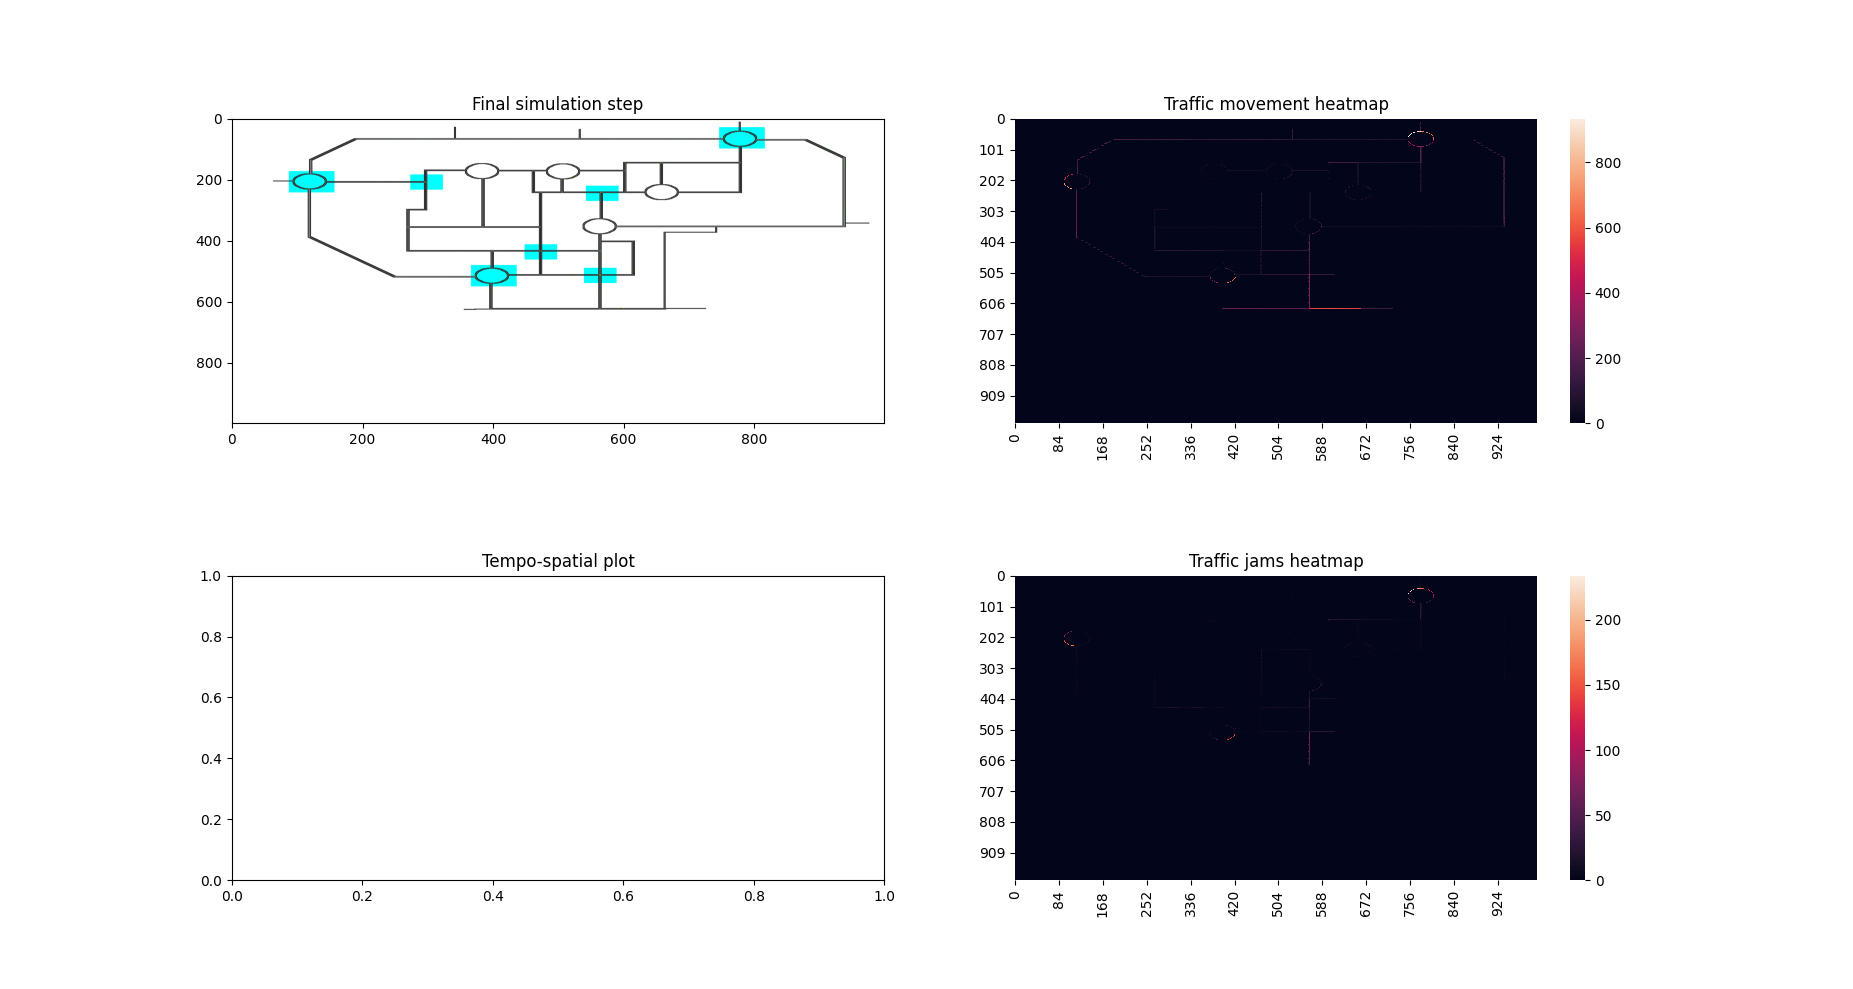
\includegraphics[width=1\textwidth]{images/5000_210.png}
    \caption{Zebrane dane dla modelu 3}
    \label{fig:dane_duzy}
\end{figure}


\section{Podsumowanie}

W pracy wykorzystano automaty komórkowe do budowania modeli i przeprowadzania symulacji. Zaimplementowano interfejs graficzny pozwalający na budowanie skomplikowanych modeli składających się z bloków takich jak pojedyncze odcinki, skrzyżowania i ronda.

Zbudowano 3 modele o różnym stopniu skomplikowano. Przeprowadzono na nich badania i zebrano dane na podstawie których wykreślono wykresy czasowo przestrzenne oraz mapy cieplne. Na podstawie zbadanych wykresów wyciągnięto wniosek, że sterowanie prawdopodobieństwami skrętów na skrzyżowaniach ma kluczowy wpływ na sterowanie natężeniem ruchu i powstawaniem zatorów. 

Wytworzone narzędzie pozwala na tworzenie skomplikowanych układów i ich badanie. Może to służyć do modelowania rozwiązań w projektowaniu miast i układów ruchów czy symulacji rozłożenia ruchu w przypadku wyłączenia drogi z użytkowania.


\bibliographystyle{unsrt}  
\bibliography{references}  %%% Remove comment to use the external .bib file (using bibtex).
%% and comment out the ``thebibliography'' section.

\end{document}
